\begin{warncard}[size=small]%
    \begin{figure}[H]
        \centering
        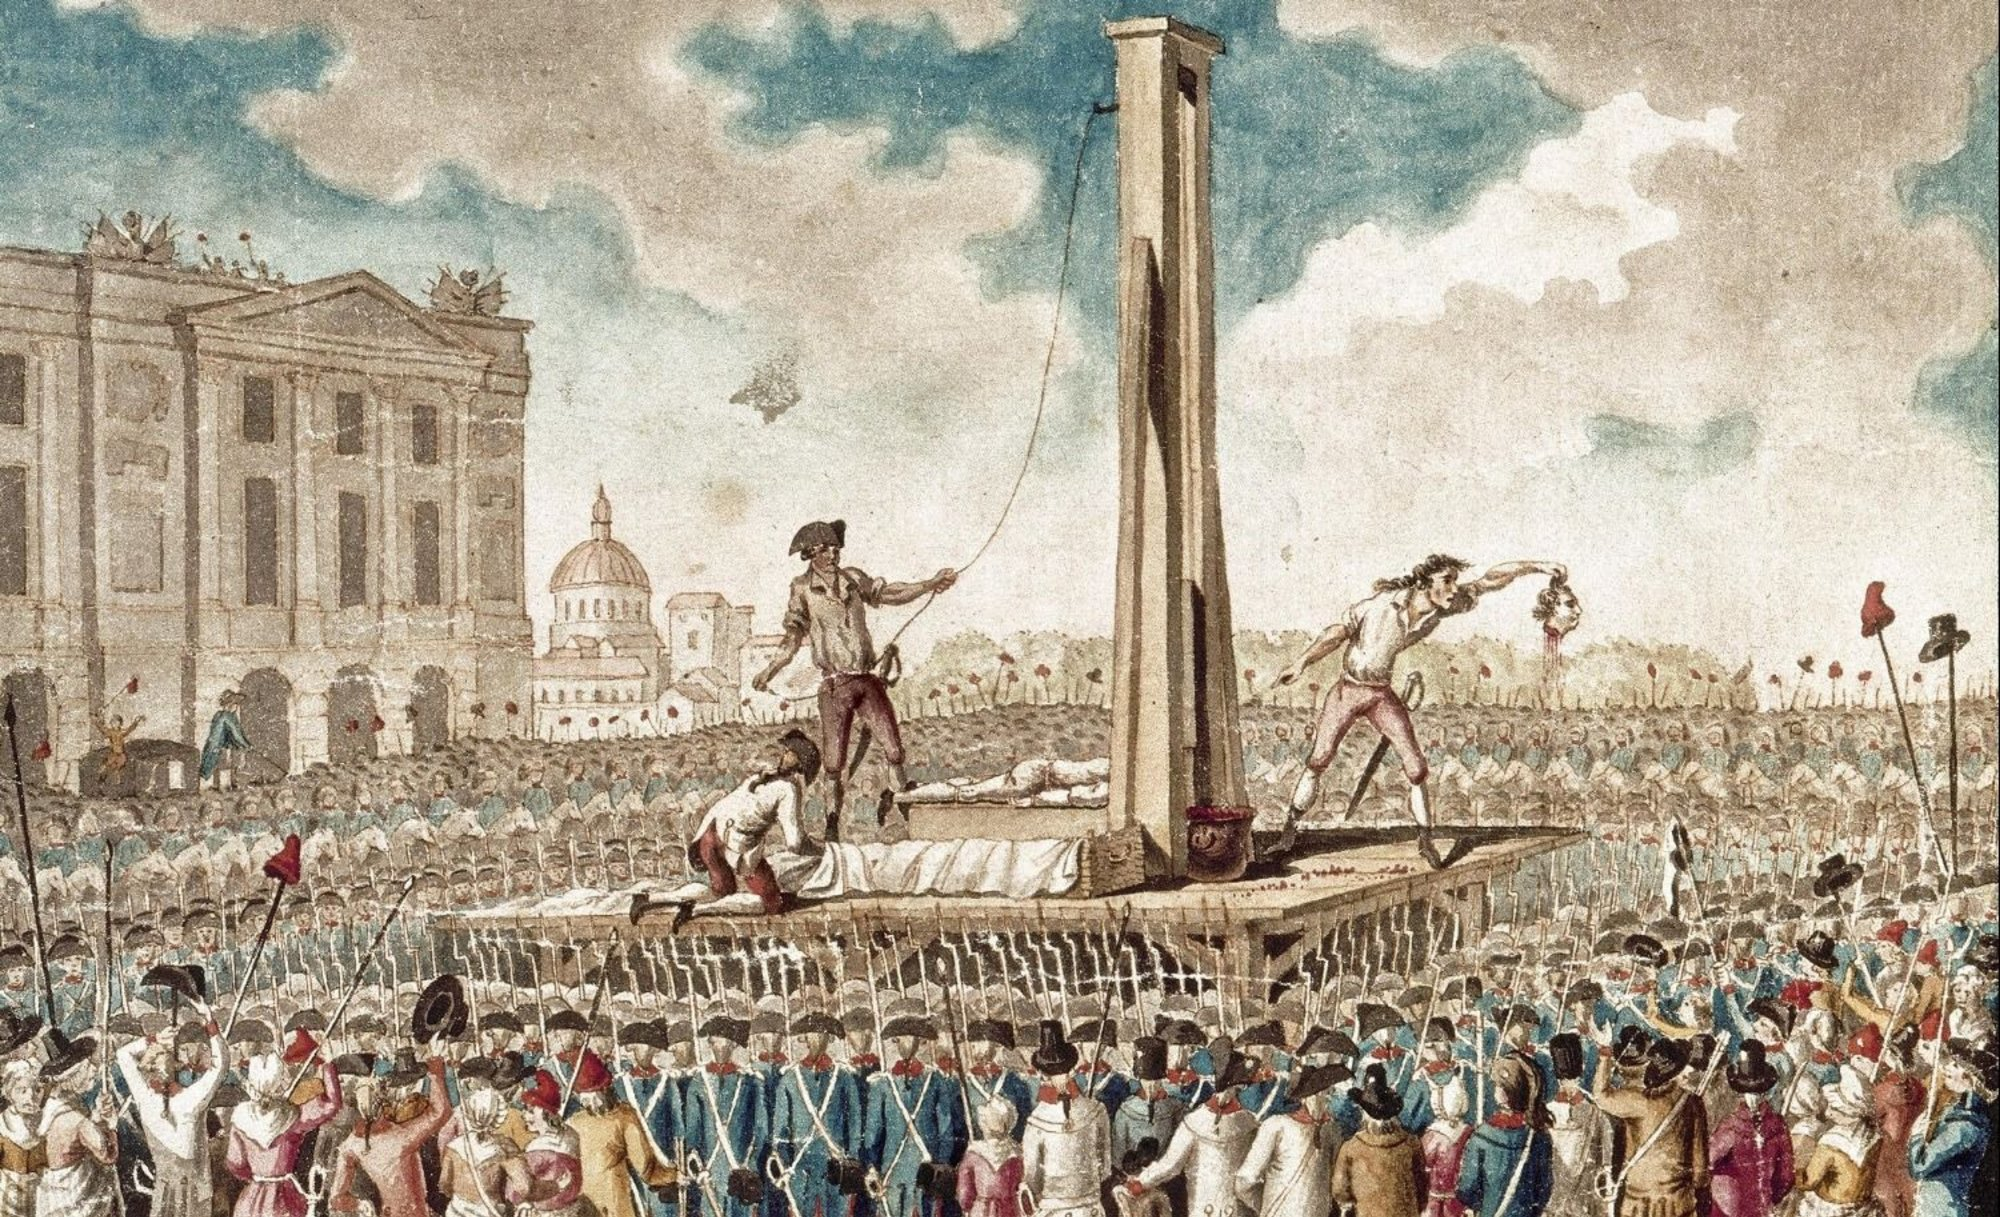
\includegraphics[width=\linewidth]{../images/decapitated}
        \caption{En 1793, Lavoisier fue arrestado por pertenecer a la Ferme Générale y, después de un juicio sumario, fue condenado a la pena de muerte. Lavoisier aprovechó lo que sería su última experiencia mundana para realizar una investigación científica. A tal fin, invitó a sus discípulos a presenciar su ejecución (llevada a cabo el 8 de mayo de 1794) como testigos del tiempo que durara moviendo los párpados después de ser decapitado. De esta forma sabrían si permanecía consciente mientras su cabeza estaba separada de su cuerpo. Con esto demostraba que la conciencia persistía por bastante tiempo después de la supuesta muerte indolora y democrática.}
        \label{fig:decapitated}
    \end{figure}
\end{warncard}